\documentclass{article}
\usepackage[T1]{fontenc}
\usepackage{lmodern}
\usepackage{graphicx}
\usepackage{amsmath,amssymb}
\usepackage[a4paper,margin=2cm]{geometry}
\usepackage[absolute,overlay]{textpos}
\setlength{\TPHorizModule}{1mm}
\setlength{\TPVertModule}{1mm}
\usepackage[indonesian]{babel}
\usepackage{hyperref}
\setlength{\emergencystretch}{2em}
% unit: Halaman 14

\begin{document}

% === Halaman 14 (llm) ===

\vspace{174.64mm}

Hitung frekuensi kemunculan huruf di dalam cipherteks tersebut sbb:\
\n\vspace{40mm}\

Jumlah total huruf, $N = 120$\n
\[ CI = \frac{\sum_{i=1}^{21} f_i(f_i-1)}{N(N-1)} = \frac{916}{120(119)} = 0,0641 \]

Nilai CI sangat dekat dengan 0,065 (teks bahasa Inggris), jauh dari 0,038 (teks acak/polyalphabetic cipher), maka kemungkinan besar ini adalah cipherteks dari \textit{monoalphabetic cipher}

% deskripsi: Dua tabel frekuensi kemunculan huruf (1-gram) yang mencakup peringkat (Rank), huruf (1-gram), jumlah absolut (Abs.), dan frekuensi relatif (Rel.)
% bbox normalisasi: [0.0480, 0.1320, 0.9520, 0.7200]
\begin{textblock*}{189.84mm}(10.08mm,39.20mm)
\noindent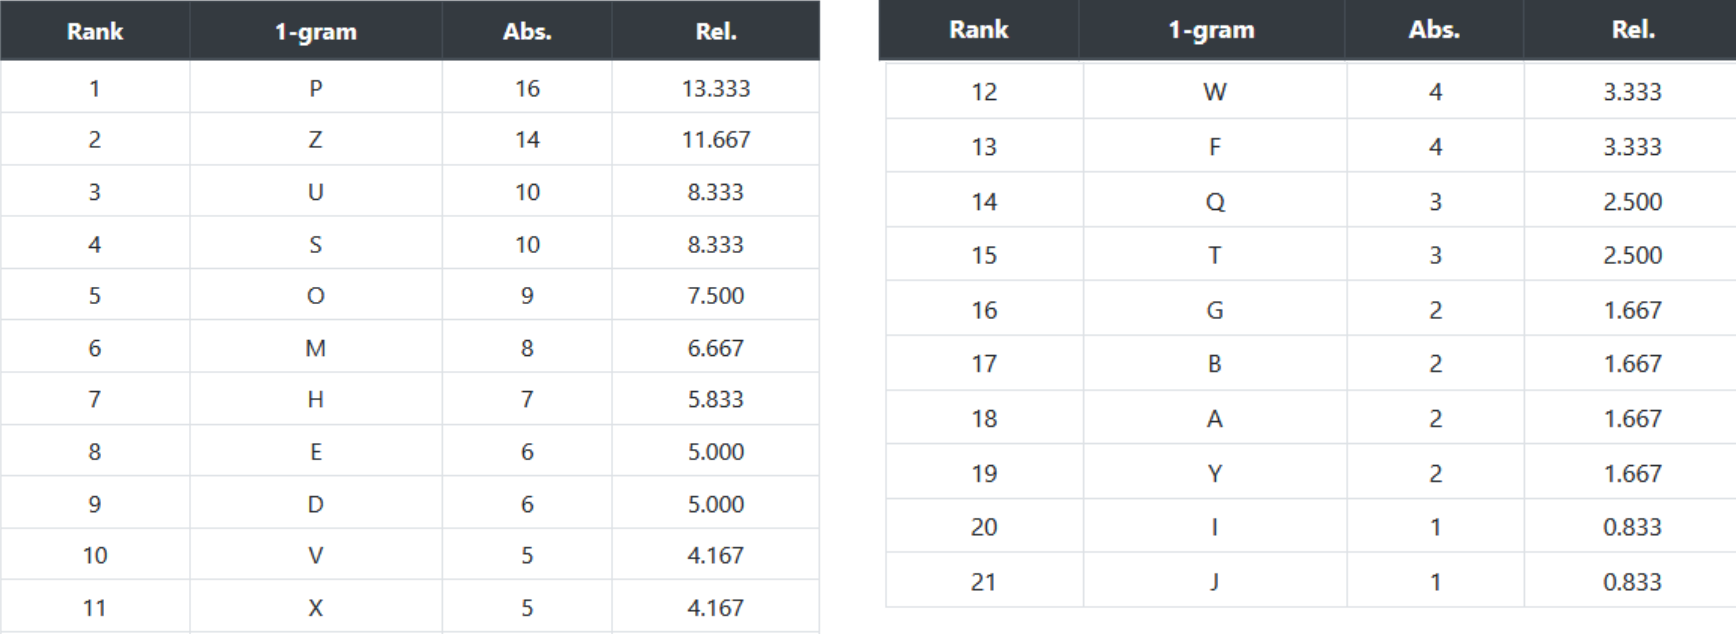
\includegraphics[width=189.84mm,height=174.64mm]{../../images/llm/page_014_img_01.png}%
\end{textblock*}

\end{document}
